\documentclass[tikz,border=5pt]{standalone}
\usepackage[T1]{fontenc}
\usepackage{lmodern,amsmath,amssymb}
\usetikzlibrary{arrows.meta,calc,positioning,fit,backgrounds,shapes.geometric,matrix,decorations.pathreplacing,patterns}
\definecolor{ink}{gray}{0.08}
\definecolor{wash}{gray}{0.965}
\definecolor{soft}{gray}{0.45}
\tikzset{box/.style={draw=ink,line width=.65pt,fill=white,align=center,inner sep=4pt,outer sep=0pt,font=\small},flow/.style={draw=ink,line width=.65pt,-{Latex[length=1.8mm,width=1.3mm]},rounded corners=2pt},annotation/.style={font=\scriptsize,text=soft,align=center},groupbox/.style={draw=soft,dashed,line width=.45pt,fill=wash}}
\begin{document}
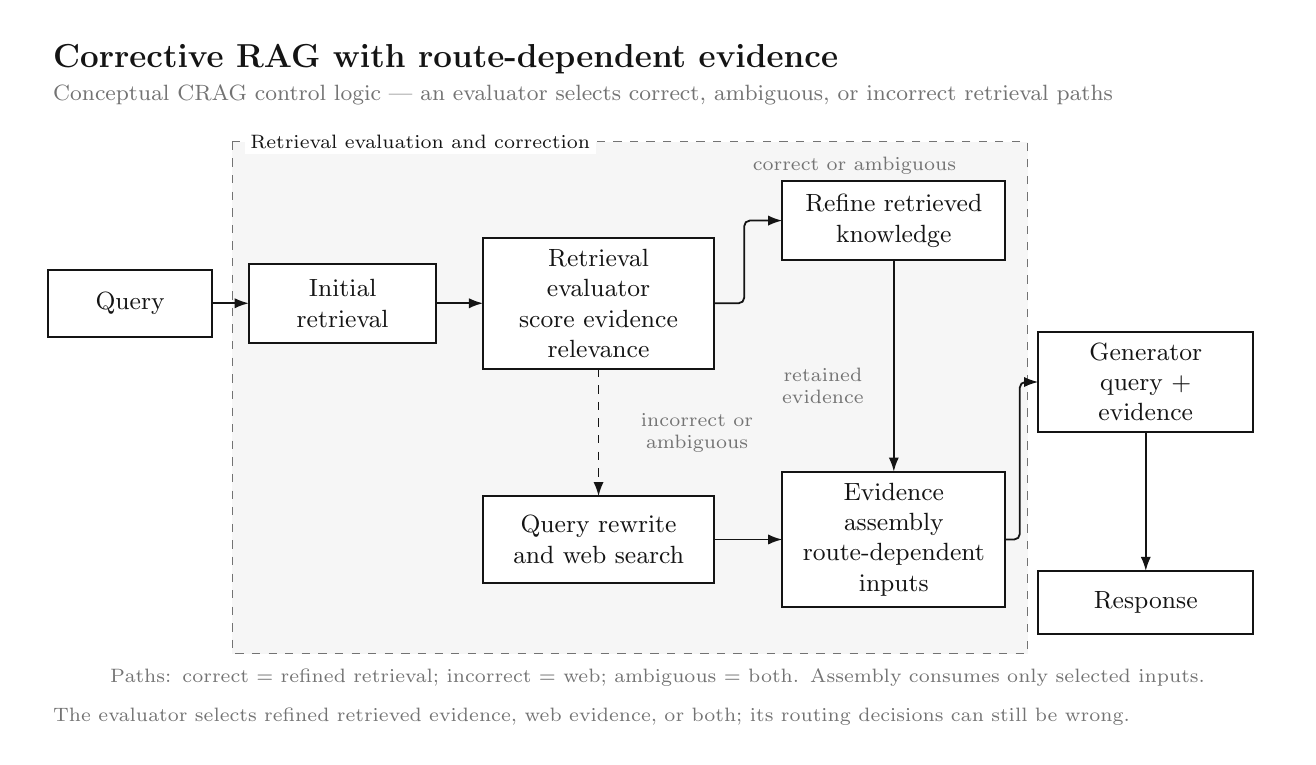
\begin{tikzpicture}[x=1cm,y=-1cm,font=\rmfamily,text=ink]

\path[use as bounding box] (0,0) rectangle (16,9);
\node[anchor=west,font=\large\bfseries] at (.2,.4) {Corrective RAG with route-dependent evidence};
\node[anchor=west,font=\footnotesize,text=soft] at (.2,.85) {Conceptual CRAG control logic | an evaluator selects correct, ambiguous, or incorrect retrieval paths};
\begin{pgfonlayer}{background}
\draw[groupbox] (2.6,1.45) rectangle (12.7,7.95);
\node[anchor=west,font=\scriptsize,fill=white,inner sep=2pt] at (2.75,1.45) {Retrieval evaluation and correction};
\end{pgfonlayer}
\node[box,minimum width=2.05cm,minimum height=0.85cm,text width=1.7999999999999998cm] (query) at (1.3,3.5) {Query};
\node[box,minimum width=2.35cm,minimum height=1.0cm,text width=2.1cm] (retrieve) at (4.0,3.5) {Initial\\retrieval};
\node[box,minimum width=2.9cm,minimum height=1.1cm,text width=2.65cm] (evaluate) at (7.25,3.5) {Retrieval evaluator\\score evidence relevance};
\node[box,minimum width=2.8cm,minimum height=1.0cm,text width=2.55cm] (refine) at (11.0,2.45) {Refine retrieved\\knowledge};
\node[box,minimum width=2.9cm,minimum height=1.1cm,text width=2.65cm] (web) at (7.25,6.5) {Query rewrite\\and web search};
\node[box,minimum width=2.8cm,minimum height=1.1cm,text width=2.55cm] (assemble) at (11.0,6.5) {Evidence assembly\\route-dependent inputs};
\node[box,minimum width=2.7cm,minimum height=1.1cm,text width=2.45cm] (generate) at (14.2,4.5) {Generator\\query + evidence};
\node[box,minimum width=2.7cm,minimum height=0.8cm,text width=2.45cm] (answer) at (14.2,7.3) {Response};
\begin{pgfonlayer}{background}
\draw[flow] (query.east) -- (retrieve.west);
\draw[flow] (retrieve.east) -- (evaluate.west);
\draw[flow] (evaluate.east) -- (9.1,3.5) -- (9.1,2.45) -- (refine.west);
\draw[flow,dashed] (evaluate.south) -- (web.north);
\draw[flow] (refine.south) -- (assemble.north);
\draw[flow] (web.east) -- (assemble.west);
\draw[flow] (assemble.east) -- (12.6,6.5) -- (12.6,4.5) -- (generate.west);
\draw[flow] (generate.south) -- (answer.north);
\end{pgfonlayer}
\node[annotation,anchor=center,text width=4.0cm] at (10.5,1.75) {correct or ambiguous};
\node[annotation,anchor=center,text width=2.0cm] at (8.5,5.15) {incorrect or ambiguous};
\node[annotation,anchor=center,text width=1.65cm] at (10.1,4.55) {retained\\evidence};
\node[annotation,anchor=center,text width=14.7cm] at (8.0,8.25) {Paths: correct = refined retrieval; incorrect = web; ambiguous = both. Assembly consumes only selected inputs.};
\node[anchor=west,align=left,font=\scriptsize,text=soft,text width=15.6cm] at (.2,8.75) {The evaluator selects refined retrieved evidence, web evidence, or both; its routing decisions can still be wrong.};
\end{tikzpicture}
\end{document}
